\section{Methoden}

\subsection{SEM}
\label{sec:SEM}

Die Rasterelektronenmikroskopie (SEM von engl. scanning electron microscopy) ist eine Technik zur hochauflösenden Untersuchung von Oberflächen.
Sie wird in vielen Feldern eingesetzt, z. B. in Medizin, Materialwissenschaften, Halbleiterindustrie und forensischen Laboren.
In \cref{fig:sem_schematic} ist schematisch ein typischer Aufbau eines SEM dargestellt.
Der auf die Probenebene fokussierte Elektronenstrahl wird rasterförmig über die Probe gefahren und verschiedene Detektoren können genutzt werden, um zeitgleich ein ortsaufgelöstes Bild der Probe aufzunehmen.
Hier können Sekundärelektronen (SE), rückgestreute Elektronen (BSE von engl. backscattered electrons), transmittierte Elektronen (STEM von engl. scanning transmission electron microscopy), Kathodolumineszenz (CL) und Röntgenstrahlung (X-ray) detektiert werden.
Mit Ausnahme von STEM befinden sich die Detektoren oberhalb der Probe, sodass nur die Oberfläche der Probe (bis zu unterschiedlicher Tiefe je nach Methode) untersucht wird und ein Dünnschnitt der Probe nicht nötig ist.

\begin{figure}[!ht]
    \centering
    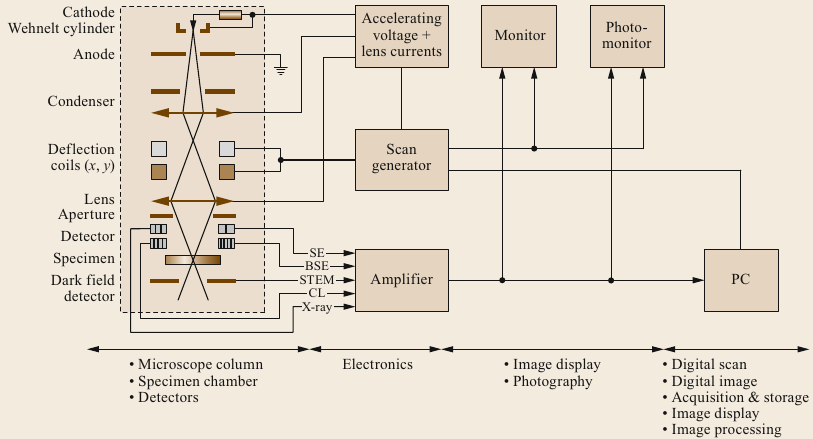
\includegraphics[width=\textwidth]{img/sem_schematic}
    \caption{
    Schematische Darstellung eines konventionellen SEM.
    Die evakuierte Mikroskopsäule (im gestrichelten Rahmen) beinhaltet die Elektronenkanone, elektromagnetische Linsen, Blenden, Probenebene und Detektoren. \cite{springer-handbook}
    }
    \label{fig:sem_schematic}
\end{figure}

Im Folgenden soll der Fokus auf Sekundärelektronen und rückgestreute Elektronen gelegt werden.
Sekundärelektronen sind dadurch definiert, dass sie eine Energie von weniger als \SI{50}{eV} haben, während rückgestreute Elektronen darüber liegen.

Rückgestreute Elektronen werden zu einem kleinen Teil dadurch erklärt, dass ein kleiner Teil der Primärelektronen mit hohem Streuwinkel $\theta > \SI{90}{\degree}$ in Richtung Elektronenkanone zurückgestreut werden und dabei wenig bis keine Energie verlieren.
Da solche Streuprozesse jedoch relativ unwahrscheinlich sind, spielen im BSE-Signal Elektronen, die nach mehreren elastischen Streuprozessen die Probe verlassen die größere Rolle.
Je nach Probeneigenschaften und Primärenergie ergibt sich eine maximale Austrittstiefe, aus der Elektronen nachgewiesen werden können.
Üblicherweise befinden sich BSE-Detektoren auf einer Seite der Elektronenkanone, sodass vornehmlich Elektronen, die in diese Richtung austreten, detektiert werden.
Da dies bei Oberflächen, die dem Detektor zugewandt sind, wahrscheinlicher ist, ergibt sich ein oberflächenorientierungsabhängiges Signal, das mit einem Schattenwurf in Lichtbildaufnahmen vergleichbar ist.
Außerdem nimmt die Wahrscheinlichkeit, dass Elektronen rückgestreut werden, mit der Ladungszahl zu, sodass BSE-Bilder chemischen Kontrast zeigen können (vgl. \cref{fig:bse-schatten}).

\begin{figure}[!ht]
    \centering
    \begin{subfigure}{0.505\textwidth}
        \centering
        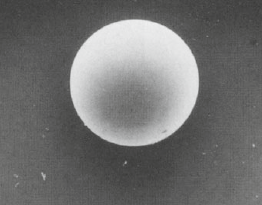
\includegraphics[width=\textwidth]{img/se-example}
    \caption{SE}
    \end{subfigure}
    %\hfill
    \begin{subfigure}{0.3\textwidth}
        \centering
        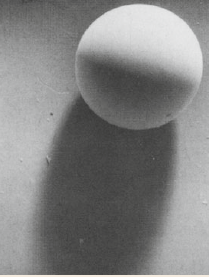
\includegraphics[width=\textwidth]{img/bse-example}
        \caption{BSE}
    \end{subfigure}
    \caption{
     SE- und BSE-Aufnahme einer \SI{1}{mm} großen Stahlkugel. \cite{springer-handbook}
    }
    \label{fig:bse-schatten}
\end{figure}

Sekundärelektronen entstehen durch inelastische Streuung hochenergetischer Elektronen mit Probenatomen.
Hierbei wird Energie auf Elektronen in der Probe übertragen, welche aus ihrem Atompotenzial gelöst werden und danach die Energiedifferenz zwischen übertragener Energie und Ionisationsenergie als kinetische Energie besitzen.
Ist die kinetische Energie ausreichend groß und findet die Ionisation ausreichend nah an der Probenoberfläche statt, kann das Elektron die Probe verlassen und nachgewiesen werden. %2nm
Flächen, die nicht senkrecht zum Primärstrahl stehen, begünstigen die Austrittswahrscheinlichkeit, wodurch SE-Bilder Informationen über die Topographie der Probe beinhalten.

Der Detektor kann sowohl das Objektivlinsensystem des Primärstrahls nutzen (through-the-lens detection) und somit parallel zum Primärstrahl messen oder seitlich montiert sein, wobei ebenfalls ein virtueller Schattenwurf erzeugt wird. \cite{springer-handbook}
In beidem Fällen wird ein Spannungsgradient verwendet, um möglichst viele Elektronen \enquote{einzusammeln}.

\subsection{Probenpräparation für SEM}
%sample preperation requirements: vakuum, conductive for sem, thin for tem etc.
%Leitfähigkeit

Zunächst einmal ist es wichtig, dass dicke Proben (z.B. ganze Insekten) mit einer leitenden Schicht (üblicherweise Gold) beschichtet werden, um elektrostatische Aufladungen der untersuchten Stelle zu verhindern.

Des Weiteren stellt sich bei biologischen Proben das Problem, dass, damit diese in die Vakuumkammer eingebracht werden können, das Wasser aus der Probe entfernt werden muss, da anderfalls die Probe ins Vakuum ausgasen würde.
Da Trocknung an der Luft häufig zu einer Zerstörung der zu untersuchenden Strukturen führt, gibt es Methoden, die Struktur der Probe während der Fixierung möglichst gut zu erhalten.

Die Methode der chemischen Fixierung verwendet verschiedene Chemikalien (u. a. Glutaraldehyd, Formaldehyd und Acrolein), um Verbindungen zwischen Aminosäuren, Proteinen und Lipiden herzustellen (üblicherweise durch kovalente Bindungen). \cite{bitesize}
Diese Chemikalien werden in einer Pufferlösung (isotonische Trägerflüssigkeit) eingebracht, um so die Morphologie der Probe zu erhalten.
Um dann das Wasser aus der Probe zu verdrängen, wird dieses zuerst langsam durch Ethanol (oder Aceton) ersetzt und dann in einer Druckkammer durch flüssiges CO$^2$.
Der Zwischenschritt über Ethanol ist nötig, da sich CO$^2$ nicht mit Wasser lösen lässt.
Dann wird ausgenutzt, dass der kritische Punkt von CO$^2$ in einer Druckkammer erreicht werden kann und hier eine Trocknung ohne Verdampung möglich ist, sodass feinporöse Strukturen nicht zerstört werden.

Da biologische Proben größtenteils aus leichten Elementen bestehen, ist in der Regel Absorption, elastische und inelastische Streuung gering, weshalb der Einsatz von Kontrastmitteln (z.B. Osmium(VIII)-oxid) nötig ist.
Diese bringen schwere Elemente (Blei, Uran, Osmium) in die Probe ein, die sich an unterschiedlichen Strukturen besser oder schlechter anlagern, und können hier als letzter Schritt aufgebracht werden.

Als Alternative zur chemischen Fixierung kann die Cryo-Fixierung genannt werden, die auf eine chemische Behandlung der Probe verzichtet, aber ein speziell dafür ausgerüstetes SEM benötigt.
Hier wird auf ein so schnelles Einfrieren der Probe gesetzt, dass keine Eiskristalle entstehen können, welche die Probenstruktur (zer-)stören könnten.

%Chemische Fixierung:
% Fixation
% Chem. Fixation
% Dehydration (ethanol, acetone)
%exchange of acetone with pressurized liquid co2
%kritisch-Punkt-Trocknung
%coating (contrast)
% SEM

%vermutlich egal, weil nicht gemacht, vielleicht nur erwähnen, dass es existiert; Vorteil=no chemical treatment:
% Cryo-Fixierung:
% Fixation
% Cryo-Fixation
% freeze-fracturing
% partial freeze-drying
% coating (contrast)
% Cryo-SEM



\subsection{TEM}

Transmissionselektronenmikroskopie (TEM) erlaubt aufgrund der geringen Wellenlänge hochenergetischer Elektronen, Auflösungen zu erreichen, die mit Lichtmikroskopie aufgrund des Abbe-Limits unmöglich sind.
So kann mittels STEM (scanning transmission electron microscopy) in kristallinen Proben subatomare Auflösung, also die Visualisierung einzelner Orbitale, erreicht werden.
Auch in biologischen Proben können mittels TEM Strukturen beobachtet werden, die im Lichtmikroskop nicht zugänglich sind.
Das TEM funktioniert sehr ähnlich zu Durchlicht-Lichtmikroskopen, wobei anstelle von Photonen Elektronen verwendet werden.
Als Elektronenquelle kann im einfachsten Fall ein Glühdraht verwendet werden und als Linsen werden Elektromagneten verwendet.
Als Bild ergibt sich so auf dem Leuchtschirm eine Abbildung der Probe, in der für Elektronen schlecht durchlässige Bereiche dunkler als durchlässigere Bereiche erscheinen.
Im Allgemeinen sind Elemente höherer Ordnungszahl schlechter durchlässig.
%Wenn der Typ STEM, Dunkelfeld gemacht hat oder sonst irgendwas spezielles, sollte ich das erwähnen, aber hat er nicht.

\subsection{Probenpräparation für TEM}
%sample preperation requirements: vakuum, conductive for sem, thin for tem etc.

Ähnlich wie in der SEM lassen sich auch hier vor allem zwei Methoden unterscheiden.

In der chemischen Methode wird zunächst Wasser in der Probe durch Aceton ersetzt.
Dann wird das Lösemittel graduell durch ein Harz ersetzt, welches die Probe aushärtet. \cite{bitesize}
Mittels eines speziellen Messers werden dann dünne Scheiben von der Probe mit einem Diamantmesser abgetrennt und auf TEM-Netze transferiert.
Dies ist nowendig, da TEM im Gegensatz zu SEM extrem dünn geschnittene Proben (etwa \SI{50}{nm} \cite{skript}) erfordert, damit ausreichend viele Elektronen die Probe durchqueren, um ein Signal zu messen.
Auch hier werden Kontrastmittel, die schwere Elemente beinhalten, aufgetragen.
% Aufbringen auf Tem-Netze

Die andere Methode ist die Cryo-Fixierung, wobei mit einer gefrorenen Probe angefangen wird, die während des Einbringens des Harzes langsam aufgetaut wird.
Dieser Prozess dauert mehrere Tage bis zu Wochen.

%Chemische Fixierung:
% 1. Fixation
% 2. Dehydration
% 3. Embedding
% 4. Thin sectioning
% 5. Staining (uranyl-acetate, lead-cytrate)

%Cryo-Fixierung
% analog, außer am anfang gefroren und ca. während embedding aufgetaut, takes days-weeks

\subsection{Astigmatismus}

Astigmatismus tritt sowohl im TEM als auch im SEM auf, wenn Elektronen in unterschiedlichen Bildrichtungen eine unterschiedliche Fokusebene haben.
Astigmatismus entsteht durch Herrstellungsfehler in den Polstücken der Linsen.
Ein hoher Astigmatismus sorgt für eine Verzerrung oder Unschärfe des Bildes in einer Bildrichtung. \cite{MyScope}
Korrigieren lässt sich Astigmatismus durch Stigmatoren (Oktupole) in Kondensator- und Objektivlinsen, mithilfe deren man ein Feld aufbaut, das diese Herrstellungsfehler ausgleicht.

%\section{Durchführung}

%actual sample preperation


%TEM:
%schwarze Punkte: schwere Elemente (OsO4 die ja vorher für Kontrast da reingepackt wurden).
	%sO4 gibt Kontraste für Lipide.
	%r mehr Kontraste: Urandingens, etc. => differential staining, differential contrast
